% Figure 2: SPC reconstruction (blue) and added uncertainty/planning (purple).
% Reconstruction follows Gaskell et al. (2023), Section 3.3.
% Camera geometry and image-to-surface associations are conditioned on.
% Covariance and the acquisition objective are an additional local analysis.
% All terrain, uncertainty bands, and camera positions are schematic.
\documentclass[tikz,border=1.5mm]{standalone}
\usepackage[T1]{fontenc}
\usepackage{amsmath,amssymb}
\usepackage{newtxtext,newtxmath}
\usetikzlibrary{arrows.meta,calc}
\definecolor{ink}{HTML}{233243}
\definecolor{muted}{HTML}{566774}
\definecolor{blue}{HTML}{347DA6}
\definecolor{bluebg}{HTML}{E4F2FC}
\definecolor{purple}{HTML}{7C65A3}
\definecolor{purplebg}{HTML}{F0E9F9}
\definecolor{teal}{HTML}{268B83}
\definecolor{orange}{HTML}{BF8531}

\newcommand{\camera}[4]{%
  \begin{scope}[shift={(#1,#2)},rotate=#3]
    \path[fill=#4!15,draw=#4,line width=.7pt,rounded corners=.4mm]
      (-.23,-.14) rectangle (.23,.14);
    \path[fill=#4!25,draw=#4,line width=.7pt]
      (-.1,-.14)--(-.17,-.27)--(.17,-.27)--(.1,-.14)--cycle;
  \end{scope}%
}
\newcommand{\card}[6]{%
  \path[draw=#5!32,fill=white,fill opacity=.34,draw opacity=1,
        line width=.55pt,rounded corners=1.4mm]
    (#1,#2) rectangle (#3,#4);
  \node[heading,anchor=west,text=#5] at ({#1+.2},{#4-.3}) {#6};
}

\begin{document}
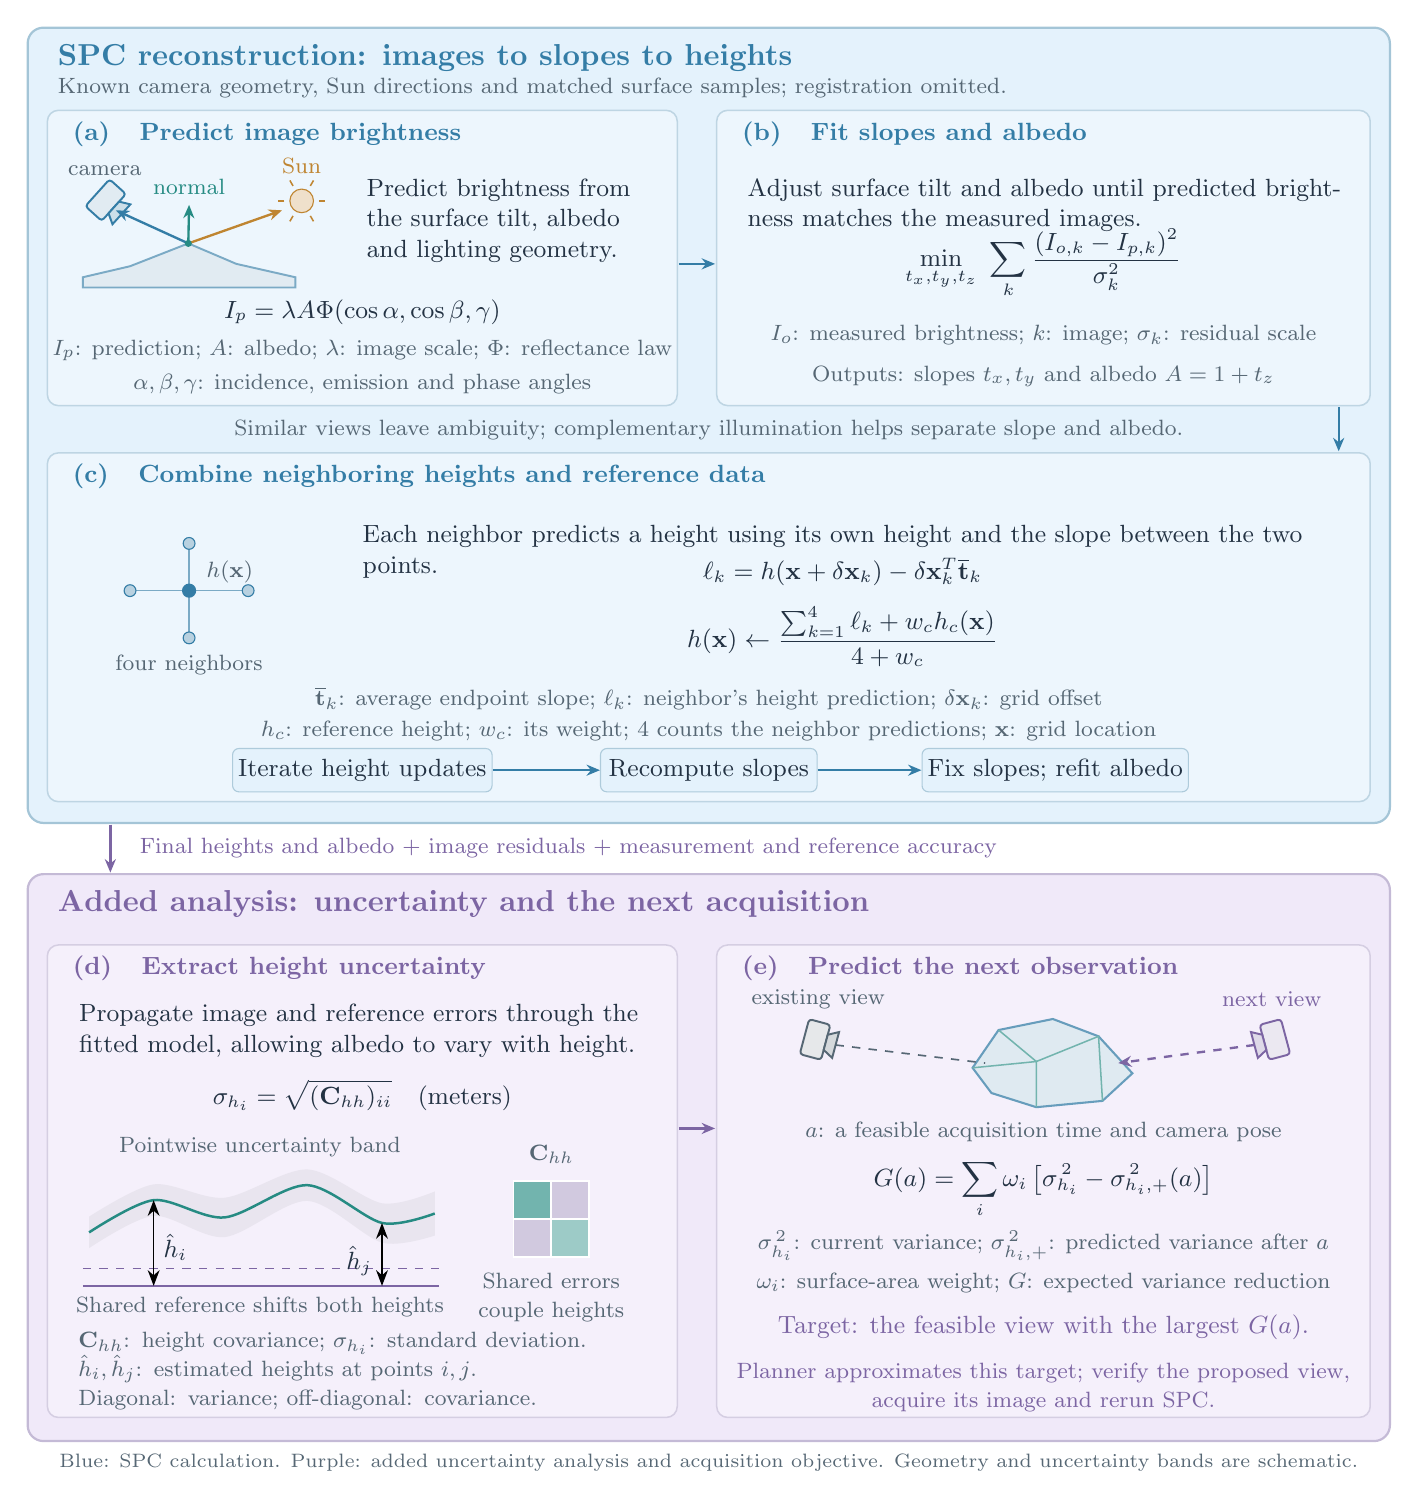
\begin{tikzpicture}[
  x=1cm,y=1cm,text=ink,font=\fontsize{9}{11}\selectfont,
  heading/.style={font=\fontsize{9.5}{11.5}\selectfont\bfseries},
  small/.style={font=\fontsize{8.5}{10.5}\selectfont,text=muted},
  tinylabel/.style={font=\fontsize{7.5}{9}\selectfont,text=muted},
  flow/.style={-{Stealth[length=1.7mm,width=1.4mm]},line width=.85pt,draw=blue},
  analysisflow/.style={flow,draw=purple},
  measure/.style={<->,>=Stealth,line width=.6pt},
  op/.style={draw=blue!40,fill=bluebg,rounded corners=.8mm,
    minimum height=.55cm,align=center,inner sep=2pt}
]
\path[use as bounding box] (0,0) rectangle (17.3,18.3);
\path[fill=bluebg,draw=blue!45,line width=.8pt,rounded corners=2mm]
  (0,8.2) rectangle (17.3,18.3);
\path[fill=purplebg,draw=purple!45,line width=.8pt,rounded corners=2mm]
  (0,.35) rectangle (17.3,7.55);
\node[font=\fontsize{11}{13}\selectfont\bfseries,text=blue,anchor=west]
  at (.26,17.92) {SPC reconstruction: images to slopes to heights};
\node[small,anchor=west] at (.26,17.53)
  {Known camera geometry, Sun directions and matched surface samples; registration omitted.};
\card{.25}{13.5}{8.25}{17.25}{blue}{(a)\quad Predict image brightness}
\card{8.75}{13.5}{17.05}{17.25}{blue}{(b)\quad Fit slopes and albedo}
\card{.25}{8.47}{17.05}{12.9}{blue}{(c)\quad Combine neighboring heights and reference data}
\draw[flow] (8.27,15.3)--(8.73,15.3);
\draw[flow] (16.65,13.48)--(16.65,12.92);

% (a) One forward equation, with its meaning and symbols nearby.
\path[fill=blue!15,draw=blue!65,line width=.7pt]
  (.7,15.13)--(1.3,15.27)--(2.04,15.56)--(2.65,15.3)--(3.4,15.13)
  --(3.4,15.0)--(.7,15.0)--cycle;
\coordinate (P) at (2.04,15.56);
\camera{.99}{16.11}{48}{blue}
\draw[flow] (P)--(1.12,15.98);
\draw[flow,draw=teal] (P)--(2.05,16.05);
\draw[flow,draw=orange] (P)--(3.23,15.98);
\fill[orange!25,draw=orange] (3.48,16.10) circle (.15);
\foreach \ang in {0,60,...,300}
  \draw[orange,line width=.55pt] ($(3.48,16.10)+(\ang:.22)$)--($(3.48,16.10)+(\ang:.3)$);
\fill[teal] (P) circle (.045);
\node[small] at (.98,16.48) {camera};
\node[small,text=teal] at (2.05,16.28) {normal};
\node[small,text=orange] at (3.48,16.55) {Sun};
\node[align=left,text width=3.5cm,anchor=north west] at (4.18,16.5)
  {Predict brightness from the surface tilt, albedo and lighting geometry.};
\node at (4.25,14.69)
  {$I_p=\lambda A\Phi(\cos\alpha,\cos\beta,\gamma)$};
\node[small] at (4.25,14.2)
  {$I_p$: prediction; $A$: albedo; $\lambda$: image scale; $\Phi$: reflectance law};
\node[small] at (4.25,13.78)
  {$\alpha,\beta,\gamma$: incidence, emission and phase angles};

% (b) Detailed normal equations are in the text, not crowded into this panel.
\node[align=left,text width=7.6cm,anchor=north west] at (9.02,16.5)
  {Adjust surface tilt and albedo until predicted brightness matches the measured images.};
\node at (12.9,15.3)
  {$\displaystyle\min_{t_x,t_y,t_z}\ \sum_k
    \frac{(I_{o,k}-I_{p,k})^2}{\sigma_k^2}$};
\node[small] at (12.9,14.4)
  {$I_o$: measured brightness; $k$: image; $\sigma_k$: residual scale};
\node[small] at (12.9,13.87)
  {Outputs: slopes $t_x,t_y$ and albedo $A=1+t_z$};
\node[small] at (8.65,13.19)
  {Similar views leave ambiguity; complementary illumination helps separate slope and albedo.};

% (c) The four-neighbor SPC relaxation, separated into explained quantities.
\begin{scope}[shift={(2.05,11.15)}]
  \foreach \dx/\dy in {-.75/0,.75/0,0/-.6,0/.6} {
    \draw[blue!65,line width=.6pt] (0,0)--(\dx,\dy);
    \fill[blue!35,draw=blue] (\dx,\dy) circle (.075);
  }
  \fill[blue] (0,0) circle (.09);
  \node[small,anchor=west] at (.1,.24) {$h(\mathbf x)$};
  \node[small] at (0,-.94) {four neighbors};
\end{scope}
\node[align=left,text width=12.2cm,anchor=north west] at (4.13,12.1)
  {Each neighbor predicts a height using its own height and the slope between the two points.};
\node at (10.35,11.39)
  {$\ell_k=h(\mathbf x+\delta\mathbf x_k)
             -\delta\mathbf x_k^T\overline{\mathbf t}_k$};
\node at (10.35,10.56)
  {$\displaystyle h(\mathbf x)\leftarrow
    \frac{\sum_{k=1}^{4}\ell_k+w_c h_c(\mathbf x)}{4+w_c}$};
\node[small] at (8.65,9.78)
  {$\overline{\mathbf t}_k$: average endpoint slope; $\ell_k$: neighbor's height prediction; $\delta\mathbf x_k$: grid offset};
\node[small] at (8.65,9.37)
  {$h_c$: reference height; $w_c$: its weight; $4$ counts the neighbor predictions; $\mathbf x$: grid location};
\node[op,minimum width=2.75cm] (height) at (4.25,8.87) {Iterate height updates};
\node[op,minimum width=2.75cm] (slope) at (8.65,8.87) {Recompute slopes};
\node[op,minimum width=2.75cm] (albedo) at (13.05,8.87) {Fix slopes; refit albedo};
\draw[flow] (height.east)--(slope.west);
\draw[flow] (slope.east)--(albedo.west);

% Outputs needed for the added statistical analysis.
\draw[analysisflow] (1.05,8.18)--(1.05,7.57);
\node[small,anchor=west,text=purple] at (1.3,7.88)
  {Final heights and albedo + image residuals + measurement and reference accuracy};
\node[font=\fontsize{11}{13}\selectfont\bfseries,text=purple,anchor=west]
  at (.26,7.17) {Added analysis: uncertainty and the next acquisition};
\card{.25}{.65}{8.25}{6.65}{purple}{(d)\quad Extract height uncertainty}
\card{8.75}{.65}{17.05}{6.65}{purple}{(e)\quad Predict the next observation}
\draw[analysisflow] (8.27,4.32)--(8.73,4.32);

% (d) The band represents pointwise uncertainty, with shared reference errors.
\node[align=left,text width=7.35cm,anchor=north west] at (.53,6.02)
  {Propagate image and reference errors through the fitted model, allowing albedo to vary with height.};
\node at (4.25,4.74)
  {$\displaystyle\sigma_{h_i}=\sqrt{(\mathbf C_{hh})_{ii}}\quad\text{(meters)}$};
\path[fill=purple!17]
  plot[smooth] coordinates {(.78,3.2) (1.6,3.61) (2.5,3.44) (3.55,3.8) (4.5,3.37) (5.17,3.52)}
  --plot[smooth] coordinates {(5.17,2.96) (4.5,2.87) (3.55,3.4) (2.5,2.94) (1.6,3.21) (.78,2.8)}--cycle;
\draw[teal,line width=.9pt]
  plot[smooth] coordinates {(.78,3.0) (1.6,3.41) (2.5,3.19) (3.55,3.6) (4.5,3.12) (5.17,3.24)};
\draw[purple,line width=.65pt] (.7,2.32)--(5.23,2.32);
\draw[purple,dashed,line width=.6pt] (.7,2.54)--(5.23,2.54);
\draw[measure] (1.6,2.32)--(1.6,3.41) node[pos=.45,right] {$\hat h_i$};
\draw[measure] (4.5,2.32)--(4.5,3.12) node[pos=.4,left] {$\hat h_j$};
\node[small] at (2.95,4.09) {Pointwise uncertainty band};
\node[small] at (2.95,2.05) {Shared reference shifts both heights};
\node[small] at (6.65,3.99) {$\mathbf C_{hh}$};
\foreach \x/\y/\tone/\shade in {0/0/teal/65,1/1/teal/45,0/1/purple/35,1/0/purple/35}
  \path[fill=\tone!\shade,draw=white,line width=.6pt]
    ({6.17+.48*\x},{3.65-.48*\y}) rectangle ++(.48,-.48);
\node[small,align=center] at (6.65,2.17) {Shared errors\\couple heights};
\node[small,align=left,text width=7.4cm,anchor=north west] at (.52,1.86)
  {$\mathbf C_{hh}$: height covariance; $\sigma_{h_i}$: standard deviation.\\
   $\hat h_i,\hat h_j$: estimated heights at points $i,j$.\\
   Diagonal: variance; off-diagonal: covariance.};

% (e) Score a future view by its predicted reduction in height variance.
\path[fill=blue!16,draw=blue!75,line width=.75pt]
  (12.0,5.09)--(12.33,5.57)--(13.02,5.71)--(13.6,5.49)
  --(14.03,5.02)--(13.65,4.67)--(12.81,4.59)--(12.24,4.77)--cycle;
\draw[teal!65,line width=.55pt] (12.33,5.57)--(12.81,5.17)--(13.6,5.49)--(13.65,4.67);
\draw[teal!65,line width=.55pt] (12.0,5.09)--(12.81,5.17)--(12.81,4.59);
\camera{10.0}{5.45}{75}{muted}
\camera{15.84}{5.45}{-75}{purple}
\draw[muted,dashed,line width=.6pt] (10.26,5.38)--(12.16,5.15);
\draw[analysisflow,dashed] (15.58,5.38)--(13.85,5.15);
\node[small] at (10.04,5.96) {existing view};
\node[small,text=purple] at (15.8,5.96) {next view};
\node[small] at (12.9,4.28) {$a$: a feasible acquisition time and camera pose};
\node at (12.9,3.55)
  {$\displaystyle G(a)=\sum_i\omega_i
    \left[\sigma_{h_i}^{\,2}-\sigma_{h_i,+}^{\,2}(a)\right]$};
\node[small] at (12.9,2.83)
  {$\sigma_{h_i}^{\,2}$: current variance; $\sigma_{h_i,+}^{\,2}$: predicted variance after $a$};
\node[small] at (12.9,2.36)
  {$\omega_i$: surface-area weight; $G$: expected variance reduction};
\node[text=purple] at (12.9,1.8)
  {Target: the feasible view with the largest $G(a)$.};
\node[small,align=center,text=purple] at (12.9,1.03)
  {Planner approximates this target; verify the proposed view,\\
   acquire its image and rerun SPC.};

\node[tinylabel] at (8.65,.08)
  {Blue: SPC calculation. Purple: added uncertainty analysis and acquisition objective. Geometry and uncertainty bands are schematic.};
\end{tikzpicture}
\end{document}
